\documentclass[11pt, a4paper]{article}
\usepackage[margin = 2cm]{geometry}
\usepackage[utf8]{inputenc}
\usepackage{setspace}
\onehalfspacing
\usepackage{graphicx}
\usepackage[left]{lineno}
\usepackage{titlesec}
\usepackage{natbib}
\titleformat{\section}{\normalfont\bfseries\large}{\thesection}{1em}{}
\titleformat{\subsection}{\normalfont\bfseries\normalsize}{\thesubsection}{1em}{}
\usepackage{ltxtable}
\usepackage[table]{xcolor}
\usepackage[T1]{fontenc} % keeps helvet from messing up \pounds
\usepackage{helvet}
\renewcommand{\familydefault}{\sfdefault}
\arrayrulecolor{gray}


\newcolumntype{L}[1]{>{\hsize=#1\hsize\raggedright\arraybackslash}X}
\newcolumntype{C}[1]{>{\hsize=#1\hsize\centering\arraybackslash}X}
\newcolumntype{R}[1]{>{\hsize=#1\hsize\raggedleft\arraybackslash}X}

\title{Project Proposal} 

\author{Anne Marie Saunders\\
	Imperial College London\\
	MSc Computational Methods in Ecology and Evolution\\
	anne.saunders19@imperial.ac.uk\\\\
	\textit{Supervisors:}\\
	Samraat Pawar, Imperial College London\\
	Lauren Cator, Imperial College London\\
	Ruiyun Li, Imperial College London\\}

\date{April 3rd, 2020}


\begin{document}

\begin{titlepage}
	\maketitle
\end{titlepage}

\textbf{Keywords:} vector abundance, time series analysis, interpolation, model selection, 

\hspace{2.1cm}vector borne disease, mosquitoes

\section{Introduction}

At the end of the 20th century, the world experienced a global resurgence of infectious disease \citep{Gubler}. Of the many diseases threatening human health, mosquito borne diseases such as malaria, yellow fever, dengue, and Rift Valley fever take millions of lives every year \citep{Yang2009}. Mosquito abundances are affected by many factors, including land-use, elevation, and vegetation cover, but meteorological variables such as temperature and precipitation in particular can be predictors of population dynamics \citep{Yoo2016}. Rainfall produces basins of water for breeding while temperature mediates life-history processes at all life stages \citep{Yang2009, Beck-Johnson2013}. Intervention in the growth of mosquito popualtions through chemical control measures is an effective public health strategy for reducing incidence of mosquito borne disease \citep{Tomerini2011}. Timing these intervention measures to interupt peak mosquito abundances can inform cost-effective disease management solutions \citep{Yang2009}. 

This investigation will 1.) Use time series analysis to assess which temporal lags of temperature and precipitation are most influential in affecting mosquito population dynamics. This will help illuminate the timing of drivers of abundance dynamics and shape models that are most predictive of abundance. Then, I will 2.) Determine which temporal scale of meteorological and count data (weekly, biweekly, or monthly) is most predictive of mosquito dynamics. This will help assess which time scale of surveillance is necessary for optimal prediction of abundances and also elucidate which time scale of prediction is most appropriate. Finally, I will 3.) Test whether the best-fit models of abundance dynamics developed through questions 1.) and 2.) are able to reliably predict abundances. This is an important step in determining whether the developed model is a useful inclusion in predictions of mosquito abundances for chemical control planning. 

%\begin{enumerate}
%	\item After what temporal lag are mosquito abundance dynamics dependent on past temperature and precipitation?
%	
%	\item What effect does interpolation between available abundance measurements have on the best-fit temporal lag of temperature and precipitation?
%	
%	\item - subject to change - How well does the best-fit model predict mosquito abundances based on time series of temperature and precipitation?
%	
%\end{enumerate}

\section{Proposed Methods}

\subsection{Temporal Lags}
Trap count data will be obtained from the VectDyn database and aggregated to each location by week. Temperature and precipitation data will be obtained from the National Oceanic and Atmospheric Administration Climate Prediction Center and mapped to each trap count location. I will then conduct model fit and selection of lagged and non-lagged models of mosquito abundance as a functions of temperature and precipitation. A final model will be produced combining the best-fit time lags of both temperature and precipitation.

%I will assess three GLM models of mosquito abundance- as a function of temperature, precipitation, and both temperature and precipitation-  using Akaike's Information Criterion (AIC) to determine which meteorological variables most commonly best describe the patterns of mosquito abundance for the datasets. I will then utilize AIC to determine the best-fit temporal lag of each meteorological variable by assessing ten separate univariate models of both temperature and precipitation lagged between zero and four weeks. The best-fit lag for each variable will be incorporated into a bivariate GLM describing mosquito abundance as a function of time-lagged temperature and precipitation.

\subsection{Interpolation}
I will then aggregate count and meteorological data to weekly, biweekly, and monthly scales. In instances where data is not fine-scaled enough to do so, data points will be interpolated through mean-filling. Model fitting and selection will then be conducted to find the best-fit temporal lag of both precipitation and temperature at each temporal scale. This can be repeated with other, lower quality, datasets where interpolation is more frequently necessitated in order to assess the effect of interpolation on model selection.

%I will then use three methods of interpolation- forward filling, backward filling, and mean filling- to interpolate count data to daily intervals. Based on these interpolated abundances, I will find the best-fit temporal lag of both temperature and precipitation for intervals between zero and twenty-eight days for each of the three interpolation techniques. I will use AIC to assess the best-fit temporal lag for temperature and precipitation for each interpolation method. These will be combined to produce three bivariate GLM models whose AICs, in combination with the AIC of the non-interpolated model, can be compared.

\subsection{Cross-Validation}  
I plan to do a leave-one-out cross validation procedure where I train the best-fit model on a collection of time series in each location as well as each temporal scale. I would then test the resultant models on a sample time series from a year that was not used to train the models. I can then assess the performance of the prediction models against the observed data. 

\section{Anticipated Outputs and Outcomes}
From my investigation, I aim to characterize the best-fit temporal lag between temperature and precipitation and mosquito population dynamics. Using interpolation at different time scales, I will be able to gain an understanding of appropriate temporal scales at which to estimate vector dynamics. I will also be able to assess the quality of abundance predictions made by different temporal scales and different extents of interpolation through cross-validation. 

\section{Project Feasibility and Timeline}

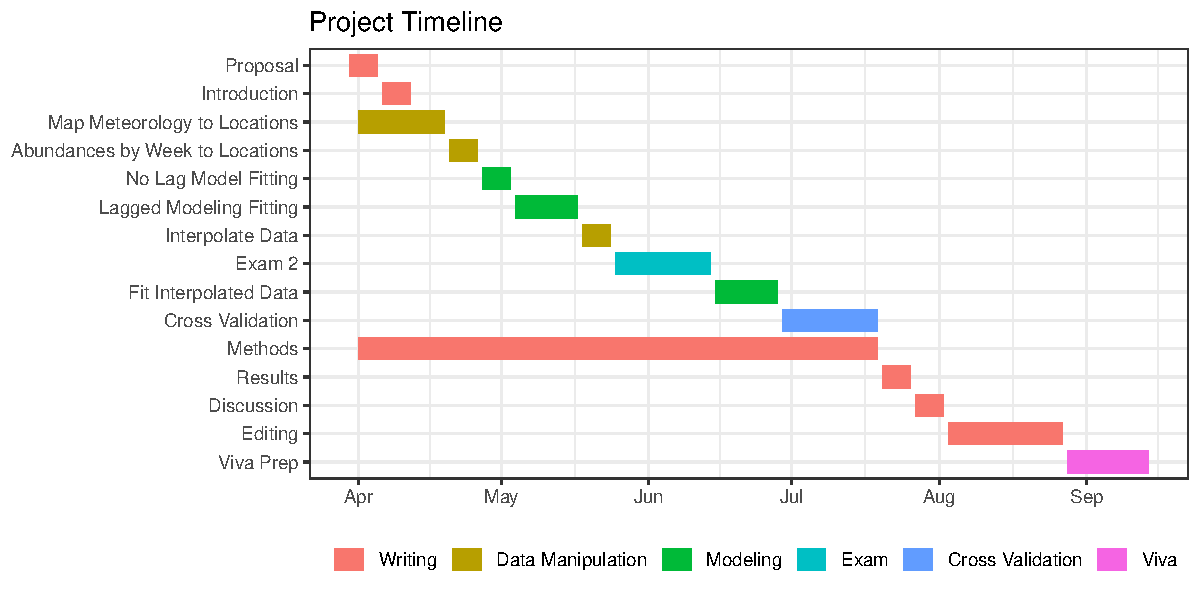
\includegraphics[height = 3.3in, width = 6.7in]{../Results/gantt.pdf}

\section{Budget}

\begin{center}
\begin{tabularx}{7in}{ L{0.6} | L{1.2} | L{0.2} }
	\textbf{Category} & \textbf{Item} & \textbf{Cost} \\\hline
	 
	 Lab Equipment & External monitor to extend my work area beyond my 13" laptop screen & \pounds 120 \\\\
	 
	 & External keyboard & \pounds 25 \
	 \\\\
	 
	 & Rechargeable batteries and charger for powering keyboard sustainably & \pounds 15

\end{tabularx}
\end{center}

\pagebreak

\topskip0pt
\vspace*{\fill}
\textbf{I have seen and approved the project and budget}

\vspace{0.8cm}
\rule{5in}{0.5pt}
\null\hfill\rule{1in}{0.5pt}

Primary Supervisor Signature
\null\hfill Date

\vspace*{\fill}
\pagebreak
\bibliographystyle{apalike}
\bibliography{Thesis.bib}

\end{document}
